\section{Fits to stress-strain curves}
PCA and logistic curve fits to the skin stress-strain curves are shown in \cref{fig:pca_fits, fig:logistic_fits}, respectively.

\begin{figure*}
    \ContinuedFloat
    \centering
    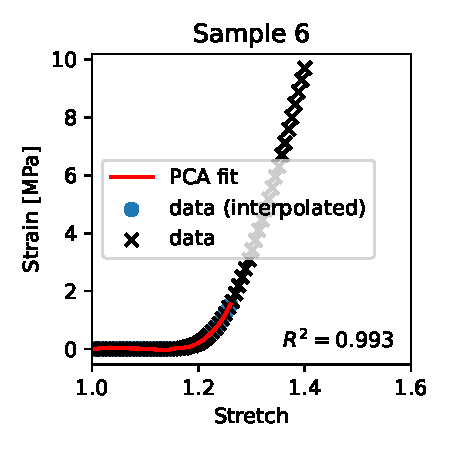
\includegraphics[width=0.24\linewidth]{skinstression/images/pca-fits/sample_6.pdf}
    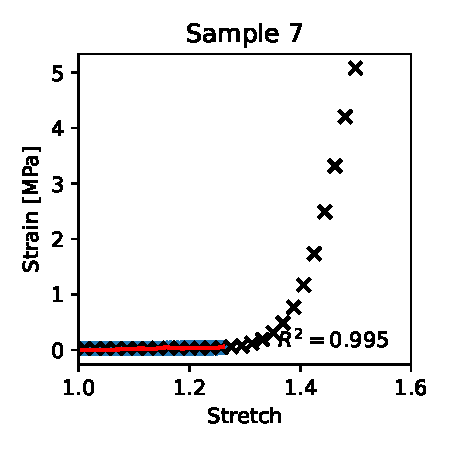
\includegraphics[width=0.24\linewidth]{skinstression/images/pca-fits/sample_7.pdf}
    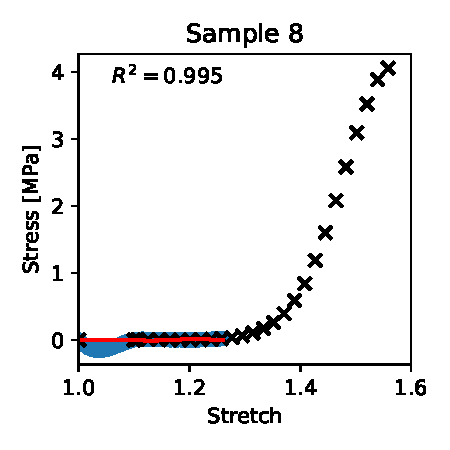
\includegraphics[width=0.24\linewidth]{skinstression/images/pca-fits/sample_8.pdf}
    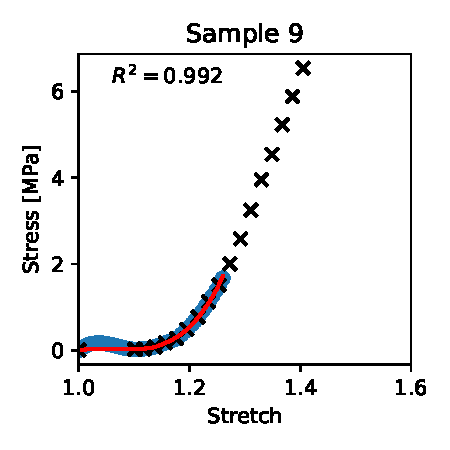
\includegraphics[width=0.24\linewidth]{skinstression/images/pca-fits/sample_9.pdf} \\
    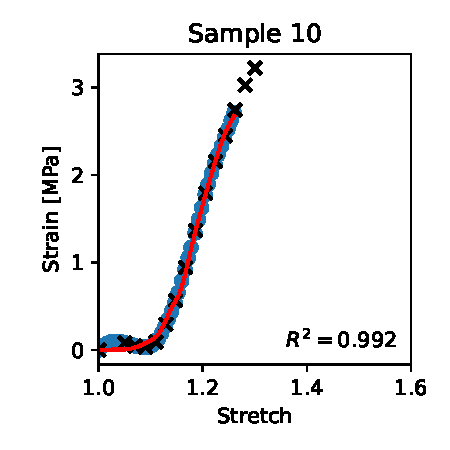
\includegraphics[width=0.24\linewidth]{skinstression/images/pca-fits/sample_10.pdf}
    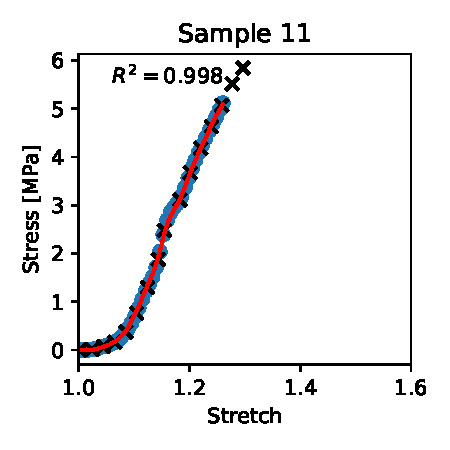
\includegraphics[width=0.24\linewidth]{skinstression/images/pca-fits/sample_11.pdf}
    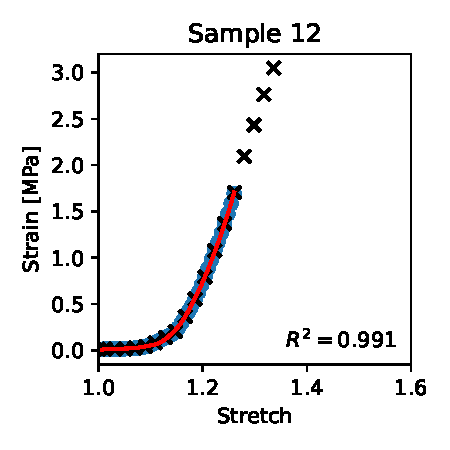
\includegraphics[width=0.24\linewidth]{skinstression/images/pca-fits/sample_12.pdf}
    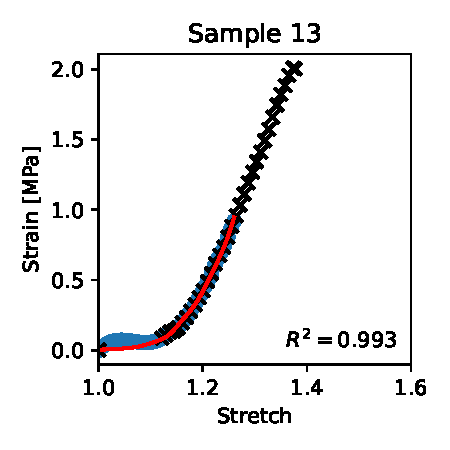
\includegraphics[width=0.24\linewidth]{skinstression/images/pca-fits/sample_13.pdf} \\
    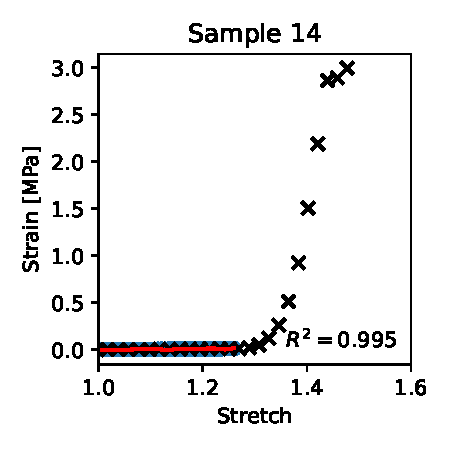
\includegraphics[width=0.24\linewidth]{skinstression/images/pca-fits/sample_14.pdf}
    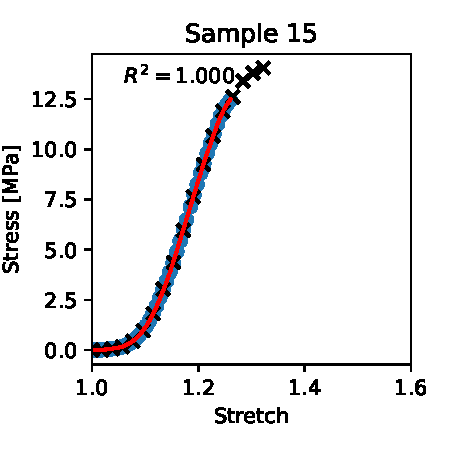
\includegraphics[width=0.24\linewidth]{skinstression/images/pca-fits/sample_15.pdf}
    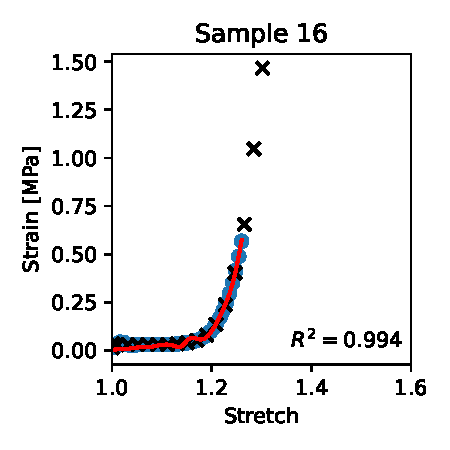
\includegraphics[width=0.24\linewidth]{skinstression/images/pca-fits/sample_16.pdf}
    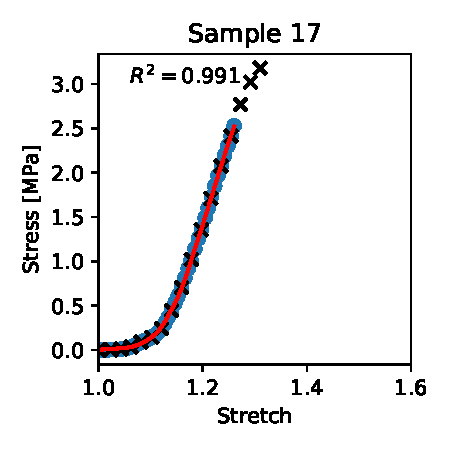
\includegraphics[width=0.24\linewidth]{skinstression/images/pca-fits/sample_17.pdf} \\
    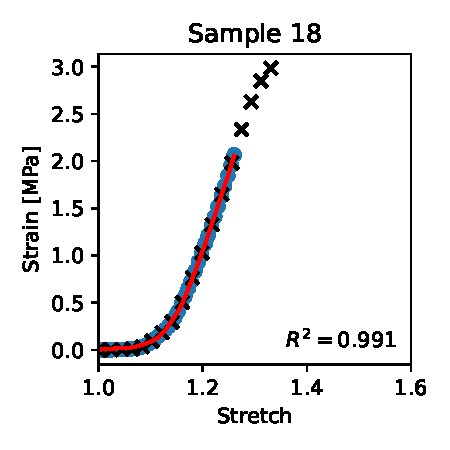
\includegraphics[width=0.24\linewidth]{skinstression/images/pca-fits/sample_18.pdf}
    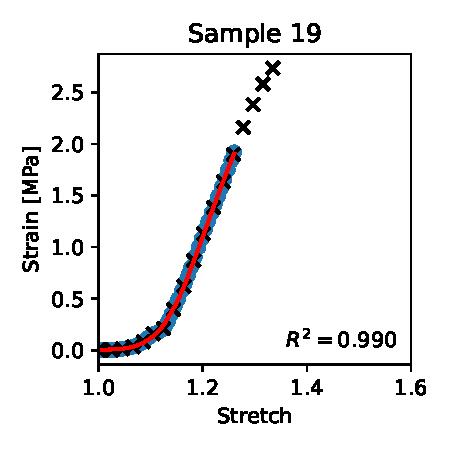
\includegraphics[width=0.24\linewidth]{skinstression/images/pca-fits/sample_19.pdf}
    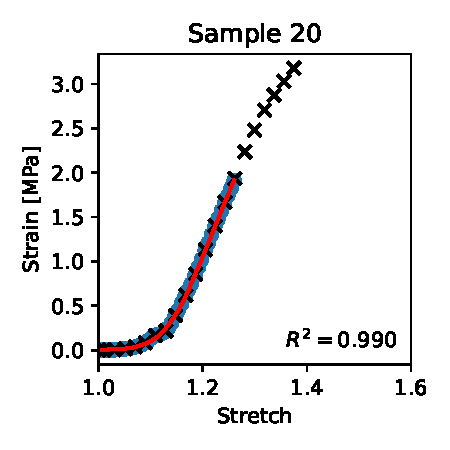
\includegraphics[width=0.24\linewidth]{skinstression/images/pca-fits/sample_20.pdf}
    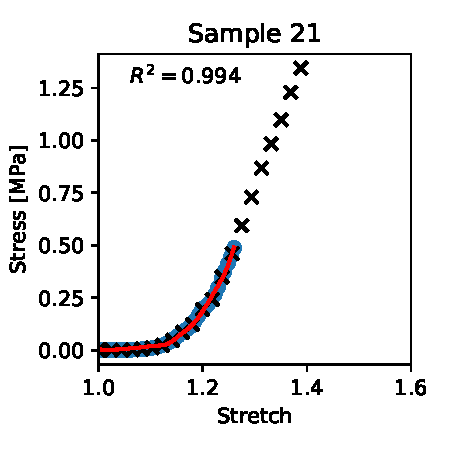
\includegraphics[width=0.24\linewidth]{skinstression/images/pca-fits/sample_21.pdf} \\
    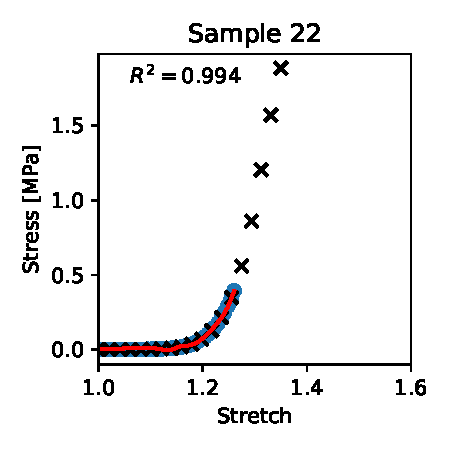
\includegraphics[width=0.24\linewidth]{skinstression/images/pca-fits/sample_22.pdf}
    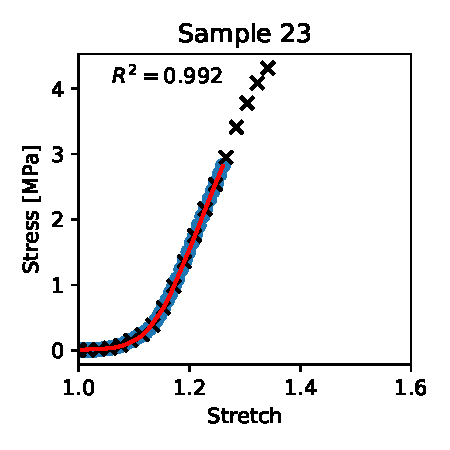
\includegraphics[width=0.24\linewidth]{skinstression/images/pca-fits/sample_23.pdf}
    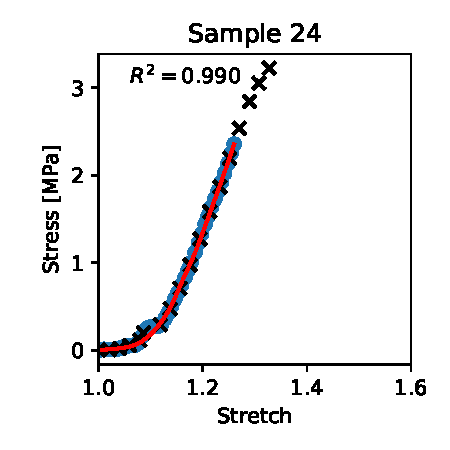
\includegraphics[width=0.24\linewidth]{skinstression/images/pca-fits/sample_24.pdf}
    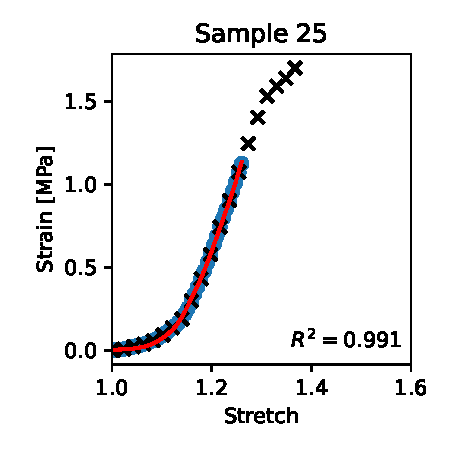
\includegraphics[width=0.24\linewidth]{skinstression/images/pca-fits/sample_25.pdf} \\
    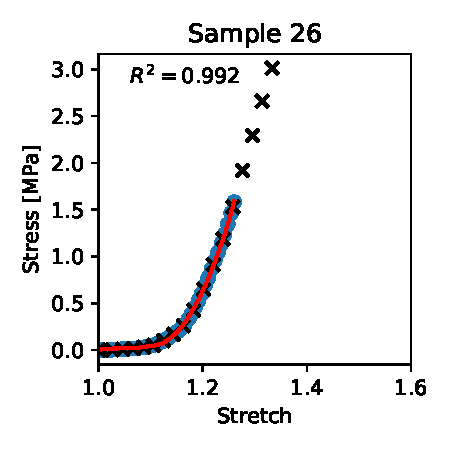
\includegraphics[width=0.24\linewidth]{skinstression/images/pca-fits/sample_26.pdf}
    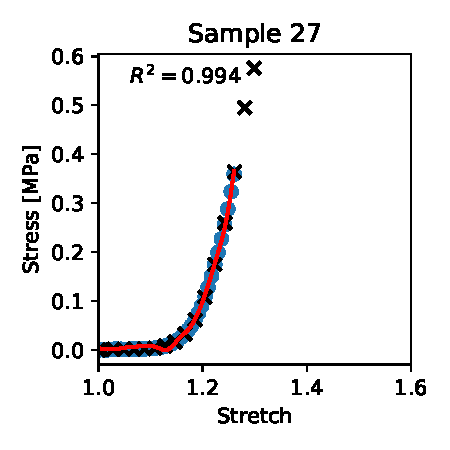
\includegraphics[width=0.24\linewidth]{skinstression/images/pca-fits/sample_27.pdf}
    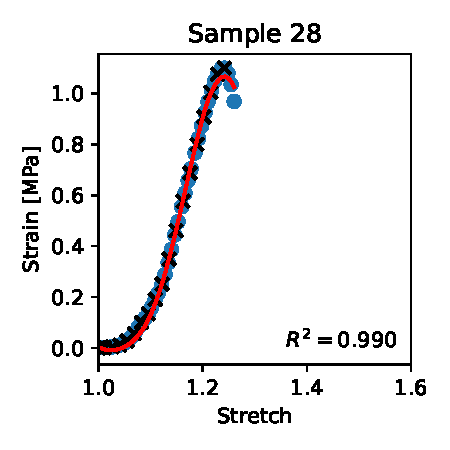
\includegraphics[width=0.24\linewidth]{skinstression/images/pca-fits/sample_28.pdf}
    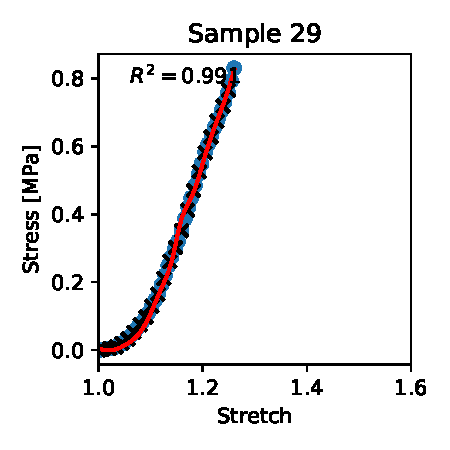
\includegraphics[width=0.24\linewidth]{skinstression/images/pca-fits/sample_29.pdf}
    \raggedleft Continued on next page.
\end{figure*}

\begin{figure*}
    \centering
    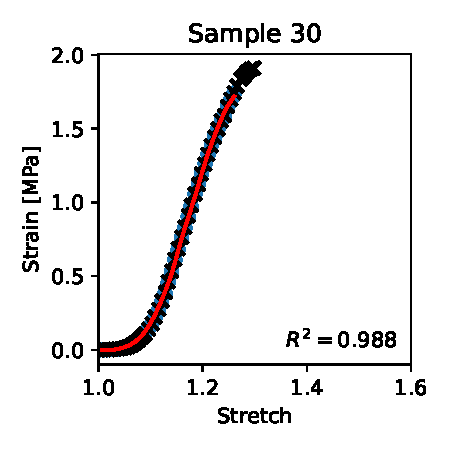
\includegraphics[width=0.24\linewidth]{skinstression/images/pca-fits/sample_30.pdf}
    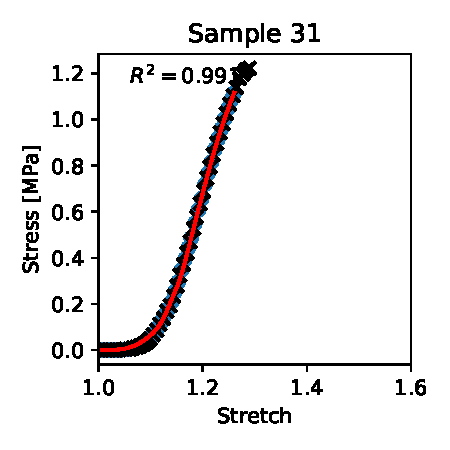
\includegraphics[width=0.24\linewidth]{skinstression/images/pca-fits/sample_31.pdf}
    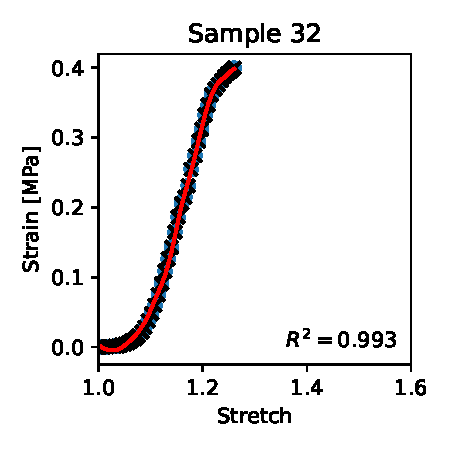
\includegraphics[width=0.24\linewidth]{skinstression/images/pca-fits/sample_32.pdf}
    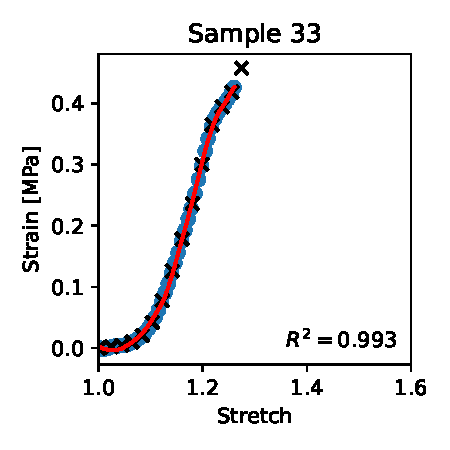
\includegraphics[width=0.24\linewidth]{skinstression/images/pca-fits/sample_33.pdf} \\
    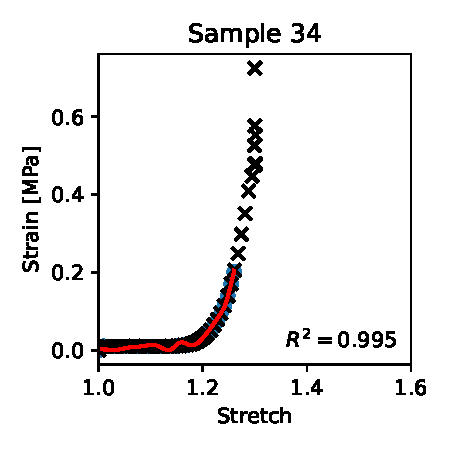
\includegraphics[width=0.24\linewidth]{skinstression/images/pca-fits/sample_34.pdf}
    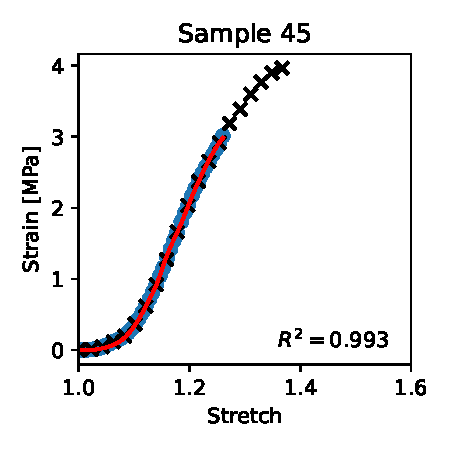
\includegraphics[width=0.24\linewidth]{skinstression/images/pca-fits/sample_45.pdf}
    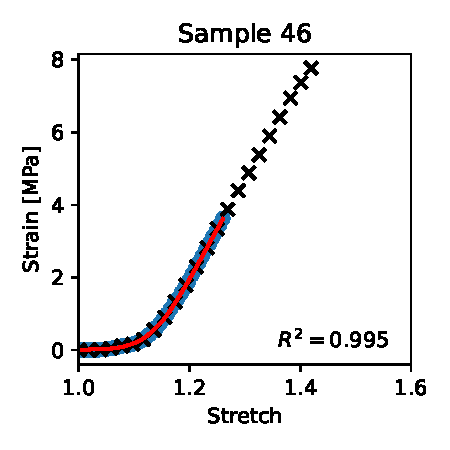
\includegraphics[width=0.24\linewidth]{skinstression/images/pca-fits/sample_46.pdf}
    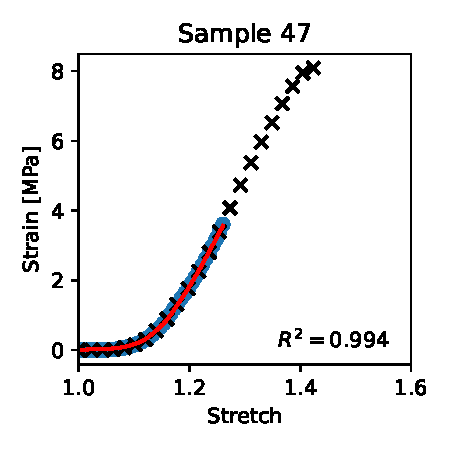
\includegraphics[width=0.24\linewidth]{skinstression/images/pca-fits/sample_47.pdf} \\
    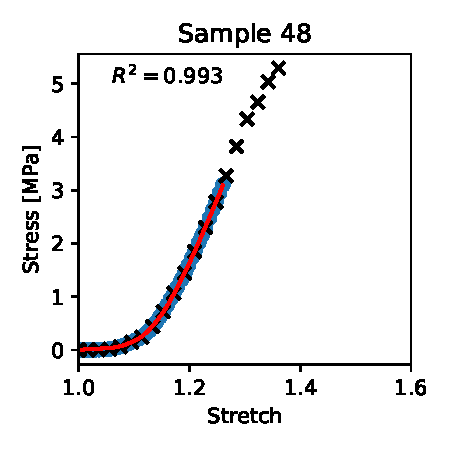
\includegraphics[width=0.24\linewidth]{skinstression/images/pca-fits/sample_48.pdf}
    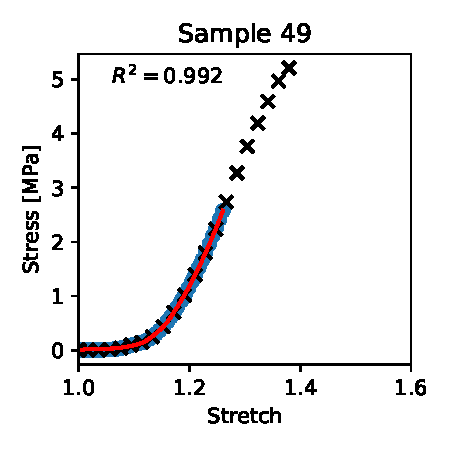
\includegraphics[width=0.24\linewidth]{skinstression/images/pca-fits/sample_49.pdf}
    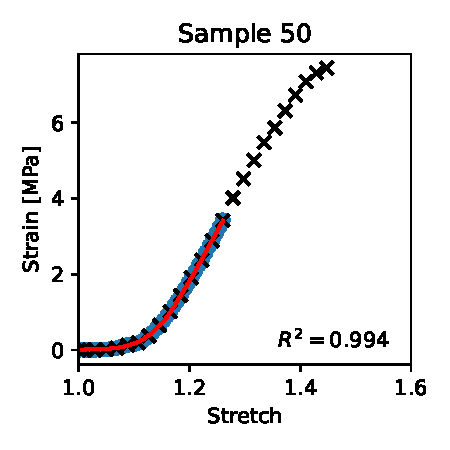
\includegraphics[width=0.24\linewidth]{skinstression/images/pca-fits/sample_50.pdf}
    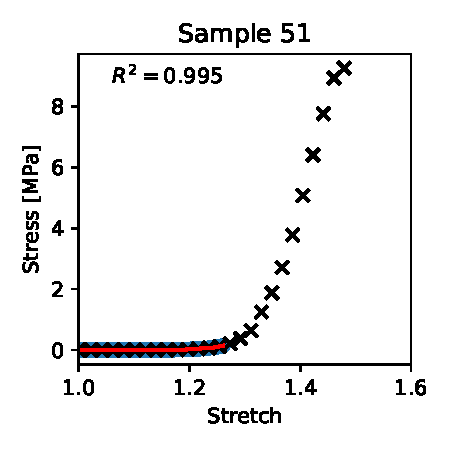
\includegraphics[width=0.24\linewidth]{skinstression/images/pca-fits/sample_51.pdf} \\
    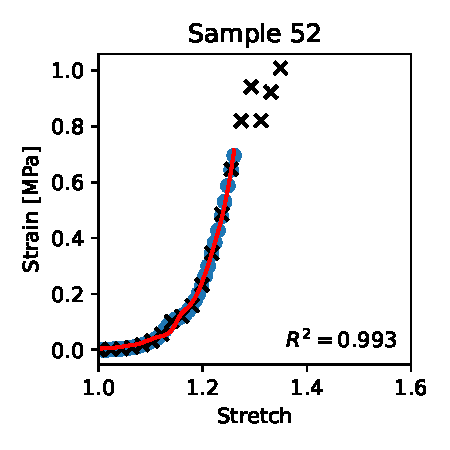
\includegraphics[width=0.24\linewidth]{skinstression/images/pca-fits/sample_52.pdf}
    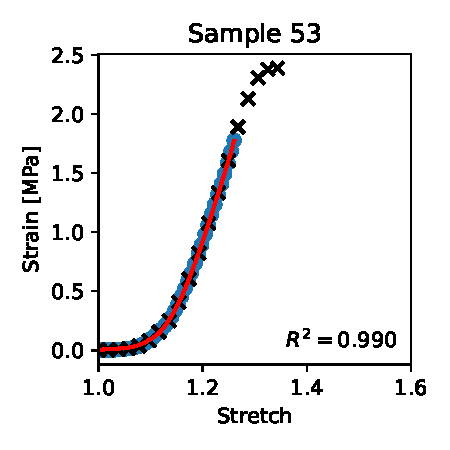
\includegraphics[width=0.24\linewidth]{skinstression/images/pca-fits/sample_53.pdf}
    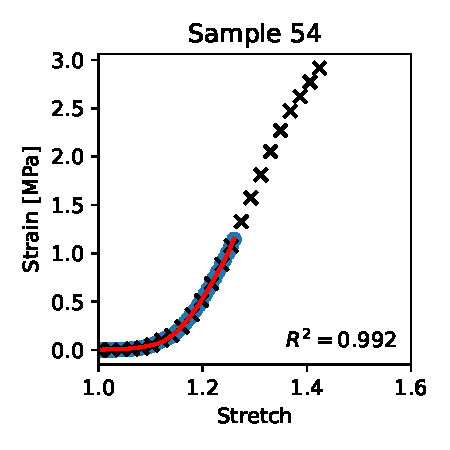
\includegraphics[width=0.24\linewidth]{skinstression/images/pca-fits/sample_54.pdf}
    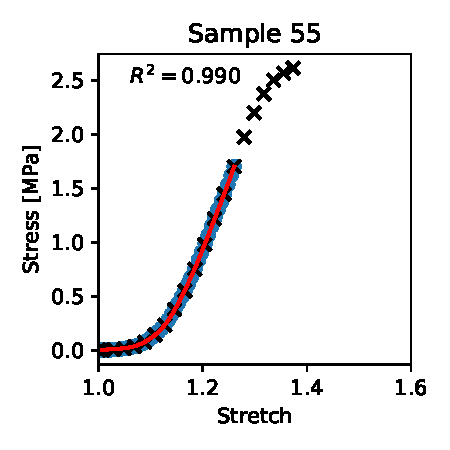
\includegraphics[width=0.24\linewidth]{skinstression/images/pca-fits/sample_55.pdf} \\
    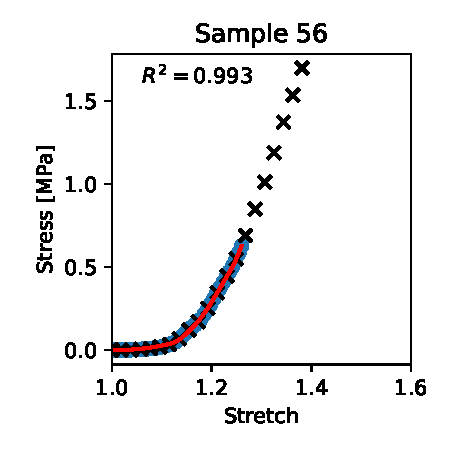
\includegraphics[width=0.24\linewidth]{skinstression/images/pca-fits/sample_56.pdf}
    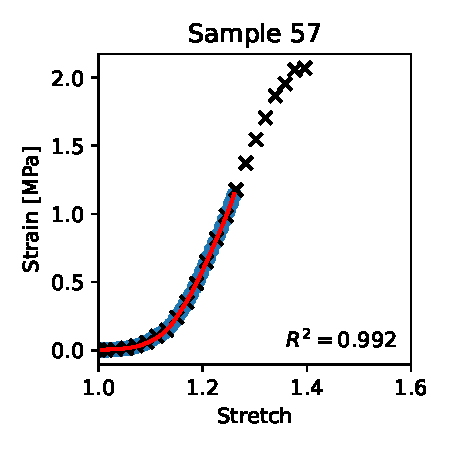
\includegraphics[width=0.24\linewidth]{skinstression/images/pca-fits/sample_57.pdf}
    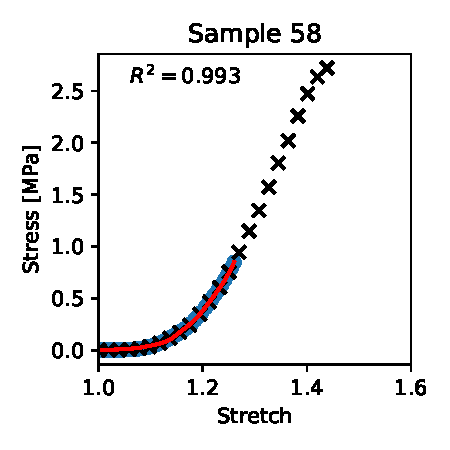
\includegraphics[width=0.24\linewidth]{skinstression/images/pca-fits/sample_58.pdf}
    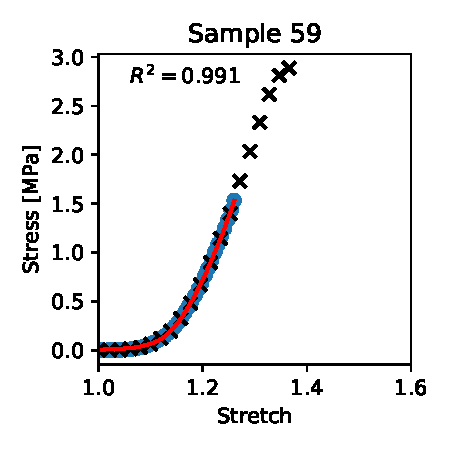
\includegraphics[width=0.24\linewidth]{skinstression/images/pca-fits/sample_59.pdf} \\
    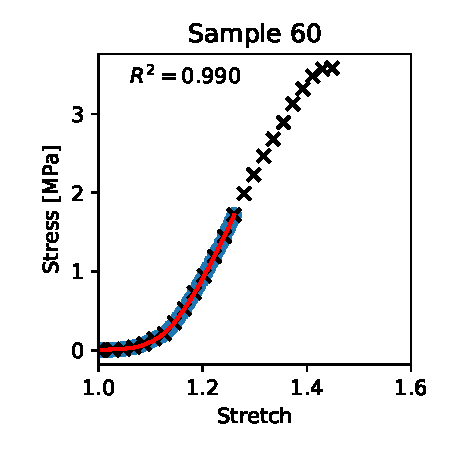
\includegraphics[width=0.24\linewidth]{skinstression/images/pca-fits/sample_60.pdf}
    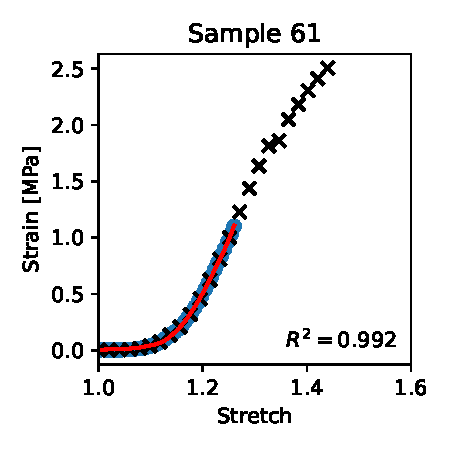
\includegraphics[width=0.24\linewidth]{skinstression/images/pca-fits/sample_61.pdf}
    \caption[PCA fits]{
        PCA fits for every truncated and interpolated strain-stress curve.
        The interpolated measurements (blue) are estimated by the PCA curve (red) along with their $R^2$.
        PCA is done on all available thigh data.
        Note that the vertical axes are not equal.
    }
    \label{fig:pca_fits}
\end{figure*}

\begin{figure*}
    \ContinuedFloat
    \centering
    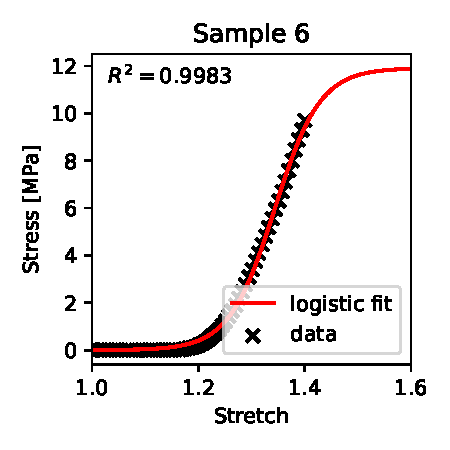
\includegraphics[width=0.24\linewidth]{skinstression/images/logistic-fits/sample_6}
    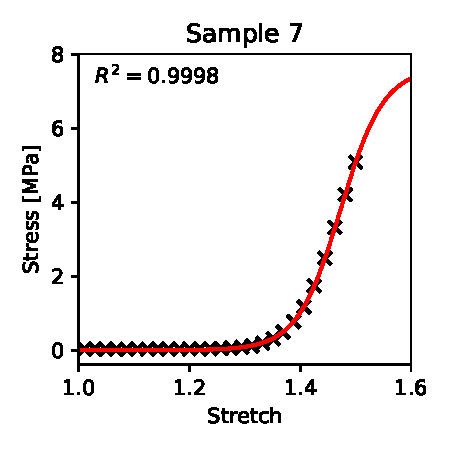
\includegraphics[width=0.24\linewidth]{skinstression/images/logistic-fits/sample_7.pdf}
    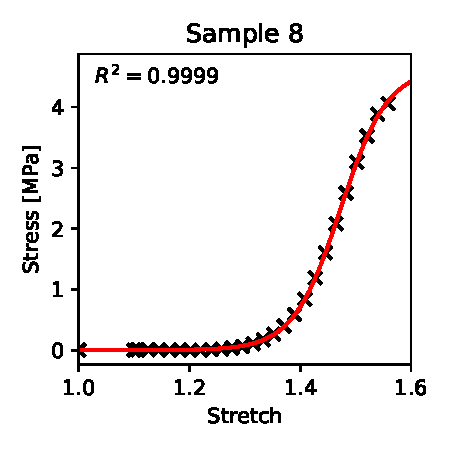
\includegraphics[width=0.24\linewidth]{skinstression/images/logistic-fits/sample_8.pdf}
    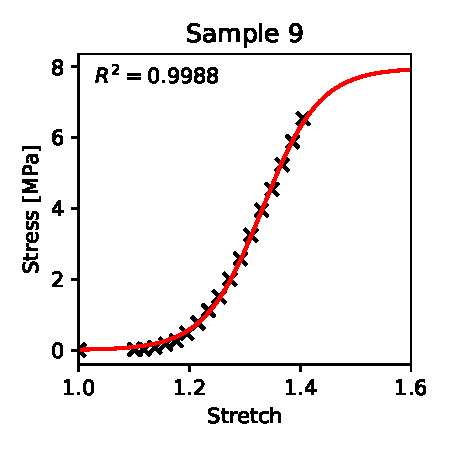
\includegraphics[width=0.24\linewidth]{skinstression/images/logistic-fits/sample_9.pdf} \\
    \includegraphics[width=0.24\linewidth]{skinstression/images/logistic-fits/sample_10.pdf}
    \includegraphics[width=0.24\linewidth]{skinstression/images/logistic-fits/sample_11.pdf}
    \includegraphics[width=0.24\linewidth]{skinstression/images/logistic-fits/sample_12.pdf}
    \includegraphics[width=0.24\linewidth]{skinstression/images/logistic-fits/sample_13.pdf} \\
    \includegraphics[width=0.24\linewidth]{skinstression/images/logistic-fits/sample_14.pdf}
    \includegraphics[width=0.24\linewidth]{skinstression/images/logistic-fits/sample_15.pdf}
    \includegraphics[width=0.24\linewidth]{skinstression/images/logistic-fits/sample_16.pdf}
    \includegraphics[width=0.24\linewidth]{skinstression/images/logistic-fits/sample_17.pdf} \\
    \includegraphics[width=0.24\linewidth]{skinstression/images/logistic-fits/sample_18.pdf}
    \includegraphics[width=0.24\linewidth]{skinstression/images/logistic-fits/sample_19.pdf}
    \includegraphics[width=0.24\linewidth]{skinstression/images/logistic-fits/sample_20.pdf}
    \includegraphics[width=0.24\linewidth]{skinstression/images/logistic-fits/sample_21.pdf} \\
    \includegraphics[width=0.24\linewidth]{skinstression/images/logistic-fits/sample_22.pdf}
    \includegraphics[width=0.24\linewidth]{skinstression/images/logistic-fits/sample_23.pdf}
    \includegraphics[width=0.24\linewidth]{skinstression/images/logistic-fits/sample_24.pdf}
    \includegraphics[width=0.24\linewidth]{skinstression/images/logistic-fits/sample_25.pdf} \\
    \includegraphics[width=0.24\linewidth]{skinstression/images/logistic-fits/sample_26.pdf}
    \includegraphics[width=0.24\linewidth]{skinstression/images/logistic-fits/sample_27.pdf}
    \includegraphics[width=0.24\linewidth]{skinstression/images/logistic-fits/sample_28.pdf}
    \includegraphics[width=0.24\linewidth]{skinstression/images/logistic-fits/sample_29.pdf}
    \raggedleft Continued on next page.
\end{figure*}

\begin{figure*}
    \centering
    \includegraphics[width=0.24\linewidth]{skinstression/images/logistic-fits/sample_30.pdf}
    \includegraphics[width=0.24\linewidth]{skinstression/images/logistic-fits/sample_31.pdf}
    \includegraphics[width=0.24\linewidth]{skinstression/images/logistic-fits/sample_32.pdf}
    \includegraphics[width=0.24\linewidth]{skinstression/images/logistic-fits/sample_33.pdf} \\
    \includegraphics[width=0.24\linewidth]{skinstression/images/logistic-fits/sample_34.pdf}
    \includegraphics[width=0.24\linewidth]{skinstression/images/logistic-fits/sample_45.pdf}
    \includegraphics[width=0.24\linewidth]{skinstression/images/logistic-fits/sample_46.pdf}
    \includegraphics[width=0.24\linewidth]{skinstression/images/logistic-fits/sample_47.pdf} \\
    \includegraphics[width=0.24\linewidth]{skinstression/images/logistic-fits/sample_48.pdf}
    \includegraphics[width=0.24\linewidth]{skinstression/images/logistic-fits/sample_49.pdf}
    \includegraphics[width=0.24\linewidth]{skinstression/images/logistic-fits/sample_50.pdf}
    \includegraphics[width=0.24\linewidth]{skinstression/images/logistic-fits/sample_51.pdf} \\
    \includegraphics[width=0.24\linewidth]{skinstression/images/logistic-fits/sample_52.pdf}
    \includegraphics[width=0.24\linewidth]{skinstression/images/logistic-fits/sample_53.pdf}
    \includegraphics[width=0.24\linewidth]{skinstression/images/logistic-fits/sample_54.pdf}
    \includegraphics[width=0.24\linewidth]{skinstression/images/logistic-fits/sample_55.pdf} \\
    \includegraphics[width=0.24\linewidth]{skinstression/images/logistic-fits/sample_56.pdf}
    \includegraphics[width=0.24\linewidth]{skinstression/images/logistic-fits/sample_57.pdf}
    \includegraphics[width=0.24\linewidth]{skinstression/images/logistic-fits/sample_58.pdf}
    \includegraphics[width=0.24\linewidth]{skinstression/images/logistic-fits/sample_59.pdf} \\
    \includegraphics[width=0.24\linewidth]{skinstression/images/logistic-fits/sample_60.pdf}
    \includegraphics[width=0.24\linewidth]{skinstression/images/logistic-fits/sample_61.pdf}
    \caption[Logistic fits]{
        Logistic fits (red) and their $R^2$ for every strain-stress curve (black).
        Note that the vertical axes are not equal.
    }
    \label{fig:logistic_fits}
\end{figure*}

\section{Configuration spaces}\label{app:skin_conf_search_spaces}
The configuration search space for Skinstression is summarized in \cref{tab:conf_skin}.

\begin{table}
    \centering
    \caption[Skinstression configuration search space]{Skinstression configuration search space.}
    \label{tab:conf_skin}
    \begin{tabular}{cccccc}
        \toprule                                                             \\
        parameter          & type    & min       & max       & step & log    \\
        \midrule                                                             \\
        weight decay       & float   & $10^{-5}$ & $10^{-4}$ & -    & \cmark \\
        learning rate      & float   & $10^{-6}$ & $10^{-2}$ & -    & \cmark \\
        $T_0$              & integer & 100       & 300       & 1    & \xmark \\
        $T_\mathrm{mult}$  & integer & 1         & 5         & 1    & \xmark \\
        $n_\mathrm{nodes}$ & integer & 64        & 128       & 64   & \xmark \\
        batch size         & integer & 8         & 64        & 8    & \xmark \\
        \bottomrule
    \end{tabular}
\end{table}

\section{Software diagrams}\label{app:skin_c4}

Communicating code can be done using the \href{https://c4model.com/}{C4 model}.
This model is an industry standard to visually communicate software architectures.
A map of the architecture can be made on four levels.
A higher level zooms in on the previous level.
The first level of the C4 model sets the context of the software.
The second level shows the high-level technical building blocks of the software.

\begin{figure*}
    \centering
    \includesvg[pretex=\small, width=\linewidth]{images/skinstression_system_context_diagram.svg}
    \caption[Skinstression system context diagram]{
        System context diagram of Skinstression.
        An experimentalist images collagen in skin tissue using an SHG microscope.
        The microscope output serves as input to Skinstression which trains a convolutional neural network to find the strain-stress curve of the imaged tissue.
        The trained model can serve as a substitution to the SHG microscope, or provide new insights in why tissue has particular stretch properties.
    }
\end{figure*}

%%% https://tex.stackexchange.com/questions/272486/fit-sidewaysfigure-to-page-width-including-caption-and-source
\begin{figure*}
    \centering
    \includesvg[pretex=\tiny, angle=90, width=0.9\textheight,height=\linewidth,keepaspectratio]{images/skinstression_container_diagram.svg}
    \caption[Skinstression container diagram]{
        Container diagram of Skinstression.
        The bounding box shows internal communications of Skinstression.
        Images generated with the SHG microscope get stored and can be read by PyimageQualityRanking (PyIQ).
        PyIQ sorts the images by quality, such that they can be read in order by notebooks and the main application.
        The main application reads locally stored configurations using Hydra.
        Trained models are stored in the model zoo.
        Hyperparameter optimizations are tracked by Optuna and stored to an SQLITE database.
        The Optuna database can be inspected by Optuna-dashboard.
        Training and hyperparameter optimization can also be inspected by Tensorboard.
        The application logs output and errors to text files.
    }

\end{figure*}